\documentclass[11pt]{article}
\usepackage[margin=1in]{geometry}
\usepackage{graphicx}
\usepackage{microtype}
\usepackage{verbatim}
\usepackage{amsmath}
\usepackage{nicefrac}
\usepackage[colorlinks=false, hidelinks]{hyperref}
\usepackage{caption}
\usepackage{subcaption}
\usepackage{listings}
\usepackage{harmony}
\usepackage{wasysym}

\begin{document}

\title{Switch Bounce \& Catch the Clown Game\\Embedded System Design, Lab 6}
\date{November 5, 2015}
\author{Ben Lorenzetti}
\maketitle

\tableofcontents

\clearpage

\section{Objectives and Problem Description}

\subsection{Does the Switch Bounce?}
\label{switch-debounce-problem-specs}

\subsection{Catch the Clown!}
\label{catch-the-clown-problem-specs}

Build a game for testing reaction times with an 8 LED rotating display,
a pushbutton trigger, and a knob for adjusting the speed/difficulty.
If the player presses the trigger in sync with
the LED display, then the display stops rotating to indicate victory.
The specifications can be summarized in the four points below:
\begin{enumerate}
\item For an 8 LED display, one LED should be illuminated at a time and
the illuminated position should rotate right one digit every period.
\item The period should be adjustable on the fly with the rotatry potentiometer knob.
\item If the user triggers the switch while the topmost (most significant bit) 
LED is illuminated, then the LED display should stop rotating
until the switch is released. The LED rotation loop should also continue--\mbox{including
through the topmost state}--if the switch is active but was triggered
during the wrong state.
\item The pushbutton switch should be debounced based on the results from
part 1.
\end{enumerate}

\section{Procedure}

\subsection{Switch Bounce}

\begin{figure}
\centering
	\begin{subfigure}[b]{.4\textwidth}
		\centering
		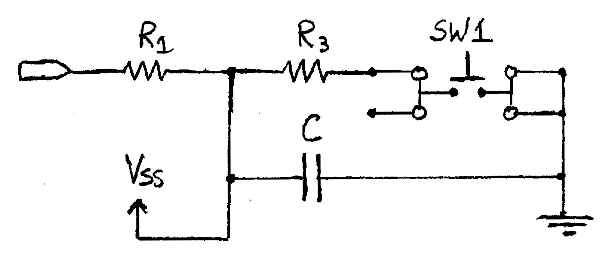
\includegraphics[width=\textwidth]{Figures/filtered-pushbutton-circuit.pdf}
		\caption[]%
		{{\small A Hardware Debounced Pushbutton: \emph{\mbox{$R_{3}$ and $C$} form a low pass filter.}}}
	\end{subfigure}
	\quad
	\begin{subfigure}[b]{0.4\textwidth}
		\centering
		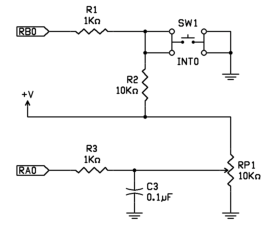
\includegraphics[width=\textwidth]{Figures/demo-board-pot-pushbutton-circuit.pdf}
		\caption[]%
		{{PIC16F887 Demo Board Schematic: \emph{pushbutton SW1 is unfiltered and requires software debouncing.}}}
	\end{subfigure}	
	\caption{Hardware vs Software Debouncing for Mechanical Switches}
	\label{io-circuit-diagram}
\end{figure}

\section{Expected Results}

\section{Experiment and Design Revisions}

\subsection{Command Line Assembly}

My \texttt{.asm} source files were assembled on the command line so
please do this if they don't compile nicely in the IDE.
On Ubuntu, with the default MPLAB installation location, 
from the directory containting \texttt{catch-the-clown.asm}, the commands are:
\begin{verbatim}
$ cp /opt/microchip/mplabx/v3.10/mpasmx/p16f887.inc ./p16f887.inc
$ /opt/microchip/mplabx/v3.10/mpasmx/mpasmx -p16f887 catch-the-clown.asm
$ more catch-the-clown.ERR
\end{verbatim}

\section{Observations}

\section{Discussion}

\clearpage

\section{Implementation Code}

\subsection{Does the Switch Bounce?}
\label{debounce-time-code}
\lstinputlisting[breaklines, basicstyle=\small]{Debounce-Time/debounce-time.asm}

\subsection{Catch the Clown!}
\label{catch-the-clown-code}
\lstinputlisting[breaklines, basicstyle=\small]{Catch-the-Clown/catch-the-clown.asm}

\end{document}
